%----------------------------------------------------------------------------------------
% PACKAGES AND OTHER DOCUMENT CONFIGURATIONS
% WARNING: Don't mess with any of the following unless you know what you are doing.
%----------------------------------------------------------------------------------------
\documentclass[english,12pt,a4paper,openany]{book}
\usepackage{datetime}
\usepackage{tabularx}
\usepackage{makecell}
\usepackage{eurosym}
\usepackage{pbox}
\usepackage[utf8]{inputenc}
\usepackage[T1]{fontenc}
\usepackage[english]{babel}
\usepackage{amsmath}
\usepackage{amsfonts}
\usepackage{fancyhdr}
\usepackage{amssymb}
\usepackage[dvipsnames]{xcolor}
\usepackage{mdframed}
\usepackage{multirow}
\usepackage{multicol} 
\usepackage{tikz}
\usepackage{graphicx}
\usepackage[absolute]{textpos} 
\usepackage{colortbl}
\usepackage{array}
\usepackage{geometry}
\usepackage{hyperref}
\usepackage{fancyhdr}
\usepackage{tabularx}
\usepackage{booktabs}
\pagestyle{fancy}
\renewcommand\headrulewidth{1pt}
\usepackage{float}
\usepackage{pdfpages}
\usepackage{tocbibind}


%------------------------------------------------------------------------------------------------------
%	The following are the RGB values for the official ATU colours.
%------------------------------------------------------------------------------------------------------	
\definecolor{ATUGreen}{RGB}{0, 91, 94}
\definecolor{ATULightGreen}{RGB}{172, 245, 189}
\definecolor{ATUNavy}{RGB}{0, 26, 121}
\definecolor{ATUOrange}{RGB}{255, 121, 30}
\definecolor{ATUPurple}{RGB}{77, 8, 87}
\definecolor{ATUSand}{RGB}{255, 232, 212}
\definecolor{ATUTeal}{RGB}{123, 185, 203}
\definecolor{ATUWarmGrey}{RGB}{200, 190, 191}
\definecolor{ATUYellow}{RGB}{248, 255, 142}



%------------------------------------------------------------------------------------------------------
%	******* CHANGE THE FOLLOWING VARIABLES
%------------------------------------------------------------------------------------------------------	

\newcommand{\reportauthor}{Rodrigo Almeida} % Change to your name
\newcommand{\projecttitle}{Biometric Data Analysis in Digital Game Scenario}
\newcommand{\reporttype}{Minor Dissertation} %Report  type (Project Plan / Final Report)
\newdateformat{monthyeardate}{\monthname[\THEMONTH], \THEYEAR}





%------------------------------------------------------------------------------------------------------	
% WARNING: Don't mess with any of the following unless you know what you are doing.
%------------------------------------------------------------------------------------------------------	
\pagestyle{fancy}
\fancyhf{}
\fancyhead[R]{\textcolor{ATUGreen}{\reportauthor}}
\fancyhead[L]{\textcolor{ATUGreen}{\projecttitle}}
\fancyfoot[L]{\textcolor{ATUGreen}{Atlantic Technological University (ATU), Galway.}}
\fancyfoot[R]{\thepage}

\begin{document}
\begin{titlepage}

\newgeometry{left=6cm,bottom=2cm, top=1cm, right=1cm}

\tikz[remember picture,overlay] \node[opacity=1,inner sep=0pt] at (2.2mm,-165mm){
\includegraphics{images/leftbar.png}}; % Fond changeable 

\fontfamily{fvs}\fontseries{m}\selectfont
\color{white}

\begin{picture}(0,0)
\put(-110,-743){\rotatebox{90}{\Huge{B.Sc. (Hons) in Software Development}}}
\end{picture}
 
\vspace{-10mm} 

\flushright 
\includegraphics[width=100mm]{images/atu-logo-green.png} 

\flushright
\vspace{10mm}
\textcolor{ATUGreen}{
\fontfamily{cmss}\fontseries{m}\fontsize{22}{26}\selectfont
\projecttitle
}
\normalsize
\color{black}

\vspace{1.5cm}
\normalsize
\textbf{By \\ \textcolor{ATUGreen}{\reportauthor}}\\ 
\vspace{15mm}
{\scshape \today} \\[0.3\baselineskip]
\vspace{75mm}
\Large {\textcolor{ATUGreen}{\textbf{{\reporttype}}}} \\
\bigskip
\normalsize
\textbf{Department of Computer Science \& Applied Physics,\\School of Science \& Computing,\\Atlantic Technological University (ATU), Galway.}\\
\end{titlepage}
\newpage
\tableofcontents
\listoffigures
\listoftables
\pagenumbering{arabic} 

%----------------------------------------------------------------------------------------
%	   ******* CHANGE the Chapters if necessary. Each chapter is encapsulated inside 
%                 its own file. The chapters below are based on the guidelines 
%                 given in the lecture.
%----------------------------------------------------------------------------------------

\chapter{Abstract}
The aim of this project is to develop a robust and enduring system using live data to analyze the correlation between a gamer's 
biometrics data and performance in a digital gaming scenario and corroborate the correlation by finding a function that approximates the relationship 
using machine learning algorithms.

Users' Biometric data were collected using a wearable device, Polar Vantage V2 and performance metrics were captured 
with a test game designed to test users' performance in a first-person shooter gaming scenario. Volunteers were selected and enrolled to gather biometric 
and test data. Heart Rate Variability, Heart Rate Average and Quality of Sleep were the biometric data collected and were used as the independent 
variables for the machine learning algorithm. The dependent variables to be predicted are the user's performance metrics in the test game. 
The performance metrics chosen were Fine Motor Average Tracking Time, Fine Motor Accuracy, Visual Average Response Time, Visual Average Tracking Time,
Visual Accuracy and Audio Average Response Time.

An on-cloud solution was proposed and implemented to access users' data and do real-time analysis. The solution was implemented using Amazon Web Services (AWS)
as the cloud provider, Amazon Relational Database Service (RDS) as a Platform as a Service (PaaS) provider and Amazon Elastic Compute Cloud (EC2) as an
Infrastructure as a Service (IaaS) provider.

Using an already predefined algorithm, a real-time model selection, hyperparameter tuning and model training pipeline were implemented to analyze the collected 
data. Various Machine Learning Models were developed and trained, enabling the team to make a strong case for correlation 
between biometric data and user performance in a digital gaming scenario. 

\chapter{Introduction}

\textbf{F}irst person shooter games represents the class of games where the  player views the environment through a viewport
and can perform such actions as looking around, moving around, aiming and firing of weapons. these actions are accomplished
using various button or combination of button.

During a typical gameplay, players are confronted with other opposing players and are required to eliminate their opponents
using various weapons available while evading enemy fire. To successfully compete in such a scenario, players are expected to
react fast, effectively track targets, accurately hit targets, perceive sound and accurately map them to a location within
their environ.

The goal of this research work is to collect biometric data from users using a Wearable Smart Watch (Polar Vantage V2)
and performance data using a Test Game designed in a first-person-shooter scenario for this purpose. This involved building
the required infrastructure to reliably collect and store users data from the various sources. Finally the data collected will be
analyzed using classical machine learning algorithm and automatic neural network to ascertain if a correlation exist between
users performance in a digital game scenario and their biometric data.


\section{Background}
PUBG: Battlegrounds (previously known as PlayerUnknown\'s Backgrounds) is a battle royale style player versus
player (PvP) shooter game developed by PUBG Studio. Players face-off with each other using various types of battlefield weapons
in a last man standing deathmatch and the last person to remain alive wins. The game is available in all major platforms
and as of March 2021, the mobile version of the game has accumulated more than a billion download outside of China with
revenue of over \$9billion while the PC and console versions have accumulated a total revenue of \$4billion
\cite{statista}.
\par
Since its first release in 2017, the game has since become one the fans favorite and has over `350,000' peak concurrent
monthly users~\footnote{statista}. As a multiple award-winning game with proven longevity records and a large community.
Interest in the game cut across different demography and is equally far-reaching across the globe.
The game playing scenario requires players to face-off with other players and there is where some skills like
`eye-hand-coordination', `ear-hand-coordination', `fine-motor' skills, etc\.. are required to compete favorably against
other players. Players have access to a varieties of weapons with different capabilities and can make in-game adjustments
to their control to suite their various preferences.

This project is a continuation of research work previously done by Fourth Year Software Design Students titled `Biometric
Data Collection for Performance Optimization in a Digital Game Scenario' in collaboration with the Department of Sports
\& Exercise Science, Atlantic Technological University.
The originating project titled \textbf{`Biometric Data Collection for Performance Optimization in a Digital
    Game Scenario'}. A desktop application Test Game designed with Unity 3D Framework and a Firestore database
that stores all user data were part of the infrastructure inherited from the previous project.

\section{Objectives}
This project aims to develop a robust and enduring system that can analyze users data on the fly using predefined machine learning
algorithm. The system is expected to function well beyond the scope of this research and expected to build better models as more data
is collected. The data collections effort involved enrolling volunteers to gather biometric and test data. Each volunteers were given
a Polar Vantage V2 Smart Watch and a Test Game  which they were expected to play daily.

\subsection{Volunteer Recruitment}
Volunteers were sought to aid the data collection effort. At the onset of the project, a total of 10 volunteers were expected to be recruited
to meet the target of 1000 data points set out as the goal to build a machine learning model. The recruitment process involved getting
ethics approval from the institution and the volunteers were expected to sign a consent form before participating in the research. 
Flyer posters were designed and distributed across the campus to attract potential volunteers. A total of 5 volunteers were eventually 
recruited and participated in the research. 

\subsection{Feature Selection}
The features selected for this research were based on the availability of data from the wearable device and the relevance of the
features to the research. The features were divided into two categories: Independent and Dependent variables. The independent
variables are the biometric data collected from the wearable device, while the dependent variables are the performance metrics


\subsubsection{Performance Metrics (Dependent Variables)}
For the purpose of measuring users performance in in a first-person shooter game scenario, three categories of metrics where
developed to measure users performance. They are listed as follows: Fine-Motor Control, Visual metrics and Audio metrics.

\textbf{Fine Motor Control}  Fine motor refers to the controlled and coordinated incremental movements made by the hand
when handling items. This metrics assesses how quickly users are able to adjust their aim to targets appearing on the screen.
Two take away from this classification is the Response Time (seconds) which quantifies reaction time and Accuracy (\%) which
quantifies users fine adjustment capabilities.

\textbf{Visual Reflexes} The game scenario under study for most of the time involves users having multiple legitimate targets
to shoot, and having to engage them simultaneously. This metrics accesses users visual reflexes by considering the Target
Accuracy which is the measure of the number of successful targets hit with the total number of target spawned expressed in
percentage. Shot Accuracy which is the measure of the number of successful shots to the number of targets hit. Finally the
Average Response Time which is the average time it takes for a target to appear before being hit.

\textbf{Audio Reflexes} User audio reflexes are accessed using the Response Time, which measures the time it takes to
identify the source of a sound within the users environment

\subsubsection{Biometric Data (Independent Variables)}
The collection and analysis of biometric data play a significant role in understanding the relationship between physical fitness and
gaming performance. This research aims to investigate how various physical parameters, such as HRV (Heart Rate Variability), Heart
Rate Max, Heart Rate average, Active Sleep and Quality of Sleep, influence a user's performance in a digital game, in this case
PUBG: Battlegrounds. The  research will also explore the potential of using biometric data to suggest the most suitable settings for
different game scenarios. By using wearable technology, which can monitor metrics such as heart rate, sleep, and activity, this study
seeks to establish a correlation between the player's physical condition and their performance in a digital game scenario. The
importance of fitness data in this context cannot be overstated. Heart Rate Variability (HRV), maximum heart rate, active sleep, and
sleep quality are all essential indicators of a person's physical condition. These metrics offers a comprehensive insight into the
user's physical condition, which can be used to improve their gaming performance.

\textbf{Heart Rate Variability (HRV):} is a measure of the variation in time between each heartbeat, and it is closely linked to
the body's stress levels. HRV is widely used as a measure of the body's autonomic nervous system, which controls the body's stress
response. A higher HRV is associated with a lower stress level, while a lower HRV is associated with a higher stress level. A research
from E. Ortega\cite{ortega2018pre} highlights the importance of HRV in sports science, as a way of understanding the psychological
state of athletes before completions. It found a positive correlation between HRV, self-efficacy, and performance among sport shooters.
Advanced shooters demonstrated lower average heart rates and employed mental skills more effectively than less experienced shooters.
This suggests HRV as a valuable asset, when transferring the psychological state of the athlete to the performance in a digital game.
It allows for a better understanding of the player's stress levels, and how it affects their performance. This personalized approach
can enhance player experience, and potentially improve their performance in the game.

The Heart Rate Variability measurements typically requires a chest strap, and measurements typically span from 5 minutes to 24 hours,
it is commonly used in clinical settings to evaluate cardiac conditions.\cite{malik1996heart} Short-term HRV analysis lasting less then
5 minutes have been proven to provide more accurate estimations compared to longer measurements.\cite{mcnames2006reliability}
Based on this, the research will focus on short-term HRV measurements, as it is more practical for the user, and it provides accurate
estimations. It will be more detailed in the methodology section.

\textbf{Heart Rate Max:} is the maximum number of times the heart can beat in a minute, and it is a measure of the body's
cardiovascular fitness. It is an important indicator of the body's physical condition, and it is used to evaluate the body's ability
to perform physical activities, reflecting their cardiovascular fitness. In this research, understanding HRmax is vital for assessing
participants fitness and endurance. It could indicates how well players can handle stress and maintain their concentration over
extended periods of time. By analysing alongside other biometric data this research could uncover valuable insight into optimizing
players performance in a digital game scenario.

\textbf{Heart Rate Average:} is the average number of times the heart beats in a minute, and it is a measure of the body's physical
activity. It is also an important indicator of the body's physical condition,     and it is another measure of the body's
cardiovascular fitness. It is used to evaluate the body's ability to perform physical activities, reflecting their cardiovascular
fitness.

\textbf{Active Step:} Active steps, as a measure of physical activity, is an important indicator of the body's physical condition. It is
used to evaluate the body's ability to perform physical activities, reflecting their cardiovascular fitness. Counting the numbers of
steps taken daily can help track overall physical activity, and it is a good indicator of the body physical condition. It is also used
to evaluate the body's ability to perform physical activities, reflecting their cardiovascular fitness.


\textbf{Quality of Sleep:} are important indicators of the body's recovery and readiness for physical activity. Active sleep is a
measure of the body's physical activity during sleep, and it is an important indicator of the body's recovery and readiness for
physical activity.High-quality sleep, marked by sufficient duration and minimal disruptions, is fundamental for overall health
impacting mood, cognitive function.  A research that evaluated Sleep and performance in Eathletes \cite{BONNAR2019647} underscores the
critical role of sleep in Eathletes performance in Esports, showing its impact on cognitive functions as a crucial factor for
competitives success. Adequate sleep improves information processing, visual motor functioning, attention, working memory, and other
functions essential for decision-making and reaction time. On the other hand, sleep depravation can significantly impair these
cognitive abilities, potentially to poor performance. For this research it proves the importance of sleep in the context of gaming
performance, and how it can be used to predict the player's readiness and tune their performance in a digital game scenario.




\subsection{Data Analysis}
Some selected features were dropped before analysis due to unavailability of data and unexpected configuration of the wearable device. The Active Steps and
Maximum heart rate were dropped from the independent variable features because unexpected configuration of the wearable required the volunteers
to manually enable some features on the device before data could be collected.
A total of 440 data points were collected from the volunteers at the time of reporting and 92 of these data points representing 21\% were deemed valid. 
Validity of data points were determined by the availability of data from the wearable device and the test game within the same time frame under 
consideration. 
Machine Learning models were designed in a pipeline to clean and normalize the data before commencement of training and other relevant analysis. 
Cleaning involves removing missing values, normalizing involves scaling the data to a range of 0 to 1 to ensure that no feature dominates and potentially 
adding bias to the model. This is particularly useful as good few of the variables where recorded in varying units. As part of the best model selection 
algorithm incorporated into the pipeline, the data is further scaled to a mean of 0 and a standard deviation of 1 for a potentially better model.

A correlation matrix was generated using the Pearson correlation coefficient algorithm to ascertain the relationship between the independent and dependent 
variables. This provided an insight into the data and certified the independence of the independent variables from each other and on the other hand shows
some level of correlation between the independent and dependent variables. These correlation were further corroborated by the machine learning models 
developed in the research to map independent variables to a dependent variable.

Best model selection was incorporated into the algorithm using the GridSearchCV algorithm from the sklearn library. It involved training various model with
a suite of M/L Algorithms (Random Forest, KNN, SVM, Logistic Regression) using various hyperparameters to determine the best model for the data. Best Model
selection decision was based on a 5-fold cross-validation technique using validation dataset. This technique was applied to the various dependent variables
to get the best performant model. An Automatic Neural Network was incorporated into the pipeline to validate the results from the classical model. This 
was done to provide a reference point to ascertain if there is likely overfitting or underfitting in the models. The Automatic Neural Network was trained
using the same data as the classical model and the results were compared to determine if both models follow the same trend. 

\subsection{Infrastructure}
The Amazon Web Services (AWS) was used to host the web application. Various services were incorporated into the system to provide all functionalities
stated. The AWS RDS configured with MySQL was used to store data in an organized form, AWS EC2 was used to provide compute time and storage for the web
application and Amazon Certificate Manager for SSL certification, Amazon Elastic Load Balancer for load balancing and Amazon Route 53 for domain name. 


\chapter{Methodology}
Describe the way you went about your project. Was your approach to the problem valid?
You need to discuss both your software development methodology and your research methodology.

\chapter{Technology Review}
This chapter is the literature review part of the dissertation and should be tightly coupled to the context and objective from the introduction.
A thorough Technology Review proves that you researched what you were doing!

\chapter{System Design}
Provide a detailed explanation of the overall system architecture \cite{lin1991divergence}, i.e. the HOW of the project.
Use UML, system architecture diagrams, screenshots, code snippets and algorithms to illustrate your design.

\section{Working with Images}
You can embed an image in a \LaTeX document using the technique shown below. System diagrams and images with a small numbers of colours (100s, not 1000s) should be stored in PNG format. Although \LaTeX doesn't care where you place your images, it is good practice to place them in a single sensible directory and apply some sort of hierarchy to them, e.g. the path images/chapter1 might contain all of the images for Chapter 1 of your dissertation.

\chapter{Machine Learning Models}

\section{Introduction}
As explained in dept in the methodology chapter, the biometric data collected through the watches generated a total of 6 independent variables:



\begin{itemize}
    \item Heart Rate Maximum \textit{bm\_HR\_max}
    \item Heart Rate Average \textit{bm\_HR\_avg}
    \item Heart Rate Variability \textit{bm\_HR\_var}
    \item Activity Steps \textit{bm\_act\_steps}
    \item Sleep \textit{bm\_sleep}
\end{itemize}

The dependent variables that were collected through the gaming tests are:

\begin{itemize}
    \item Fine Motor Average Tracking Time \textit{fm\_avg\_trk\_time}
    \item Fine Motor Accuracy \textit{fm\_accuracy}
    \item Visual Average Response Time \textit{vx\_avg\_res\_time}
    \item Visual Shot Accuracy \textit{vx\_shot\_accuracy}
    \item Visual Target Accuracy \textit{vx\_trg\_accuracy}
    \item Audio Average Response Time \textit{au\_avg\_res\_time}
\end{itemize}

The goal based on the research question was to find the correlation between the independent and dependent variables. When approaching a machine learning problem, one of the fundamental
considerations is whether the problem is a regression or classification problem.

\subsection*{Classification vs Regression Problem}
The main difference between a classification and regression problem is the type of dependent variable. The dependent variable, can be one or more, and they are the variables that are being predicted. In
classification, the dependent variable is categorical, meaning it can take one of a limited number of values. Examples includes predicting whether an email is spam or not,
predicting whether a patient has a disease or not. In regression, the dependent variable is continuous and numerical, meaning it can take any value within a range. Examples
includes predicting house prices, stock prices, temperature. In this project, the dependent variables are continuous and numerical, making it a regression problem. The goal
was to predict the dependent variables based on the biometric data collected from the watches.





\chapter{Conclusion}

The project was concluded successfully, and the team was able to deliver a working solution to the client's requirements. An enduring
solution capable of processing real-time data and on the fly was deployed to run a machine learning algorithm to predict user performance
based on their biometric data. Several challenges were encountered during the project because of limited resources available to the team
which meant discarding some industry-standard tools that could not work with the available resources. The chosen Virtual Machine (EC2 Micro)
has a capacity of 1GB RAM and 1 CPU, which was not enough to deploy an Angular Application and Docker. From the results of the analysis, the team
was able to show that there is a strong indication of correlation between the biometric data and the user performance. However, insufficient data
meant that the model could not be trained to a high degree of accuracy, and it is the opinion of the team that with more data, the model could only 
get better.


\subsubsection*{Otito}
This project was a great learning experience for me and an opportunity to work with various technologies. I was able to learn and understand how 
cloud-based web applications and services are developed and deployed. This project also gave me the opportunity to work with a client and understand 
the implications of changing requirements and how to adapt to them in a software development environment. I personally enjoyed working with the team and 
from a personal perspective, I strongly believe that the project was a success and it was down to everyone's hard work and dedication, and very proud of 
the work and ingenuity shown by the team in problem-solving. 

\subsubsection*{Rodrigo}

The journey through the project has been a challenging and rewarding experience. It gave me the opportunity to collaborate directly with a client and develop 
a solution that has real-world applications. I had the opportunity to work with technologies that were new to me, giving me the unique chance to expand my skill 
set, particularly in the areas of data analysis, machine learning, and cloud computing which is a field that we have not extensively covered in our course.  
This project brought to light the complexities involved in real-time data analysis and the design of robust system architectures. It reinforced the
importance of interdisciplinary knowledge and the integration of diverse technologies to address a complex real-world problem effectively. 
The collaboration between the team members was excellent, and we were able to combine our individual strengths to deliver a high-quality solution. 
The project was a valuable learning experience, and I am proud of the work we have accomplished.



\subsubsection*{Otito}
\chapter{Appendices}

\label{appendix}



\label{sec:github-links}
\addcontentsline{toc}{section}{Appendix A: GitHub Repositories Links}

The following are the links to the GitHub repositories for the project:

\begin{itemize}
    \item \textbf{Frontend Repository:} \\ \url{https://github.com/rodAlm08/exec_dash.git}
    \item \textbf{Backend Repository:} \\ \url{git@github.com:intotito/applied_project.git}
    \item \textbf{Documentation Repository:} \\ \url{https://github.com/rodAlm08/Final_Project_Dissertation.git}
    \item \textbf{Abandoned Frontend Repository:} \\ \url{https://github.com/rodAlm08/Executive_Dashboard.git}
\end{itemize}




\label{sec:ethics-application}
\addcontentsline{toc}{section}{Appendix B: Ethics Application}
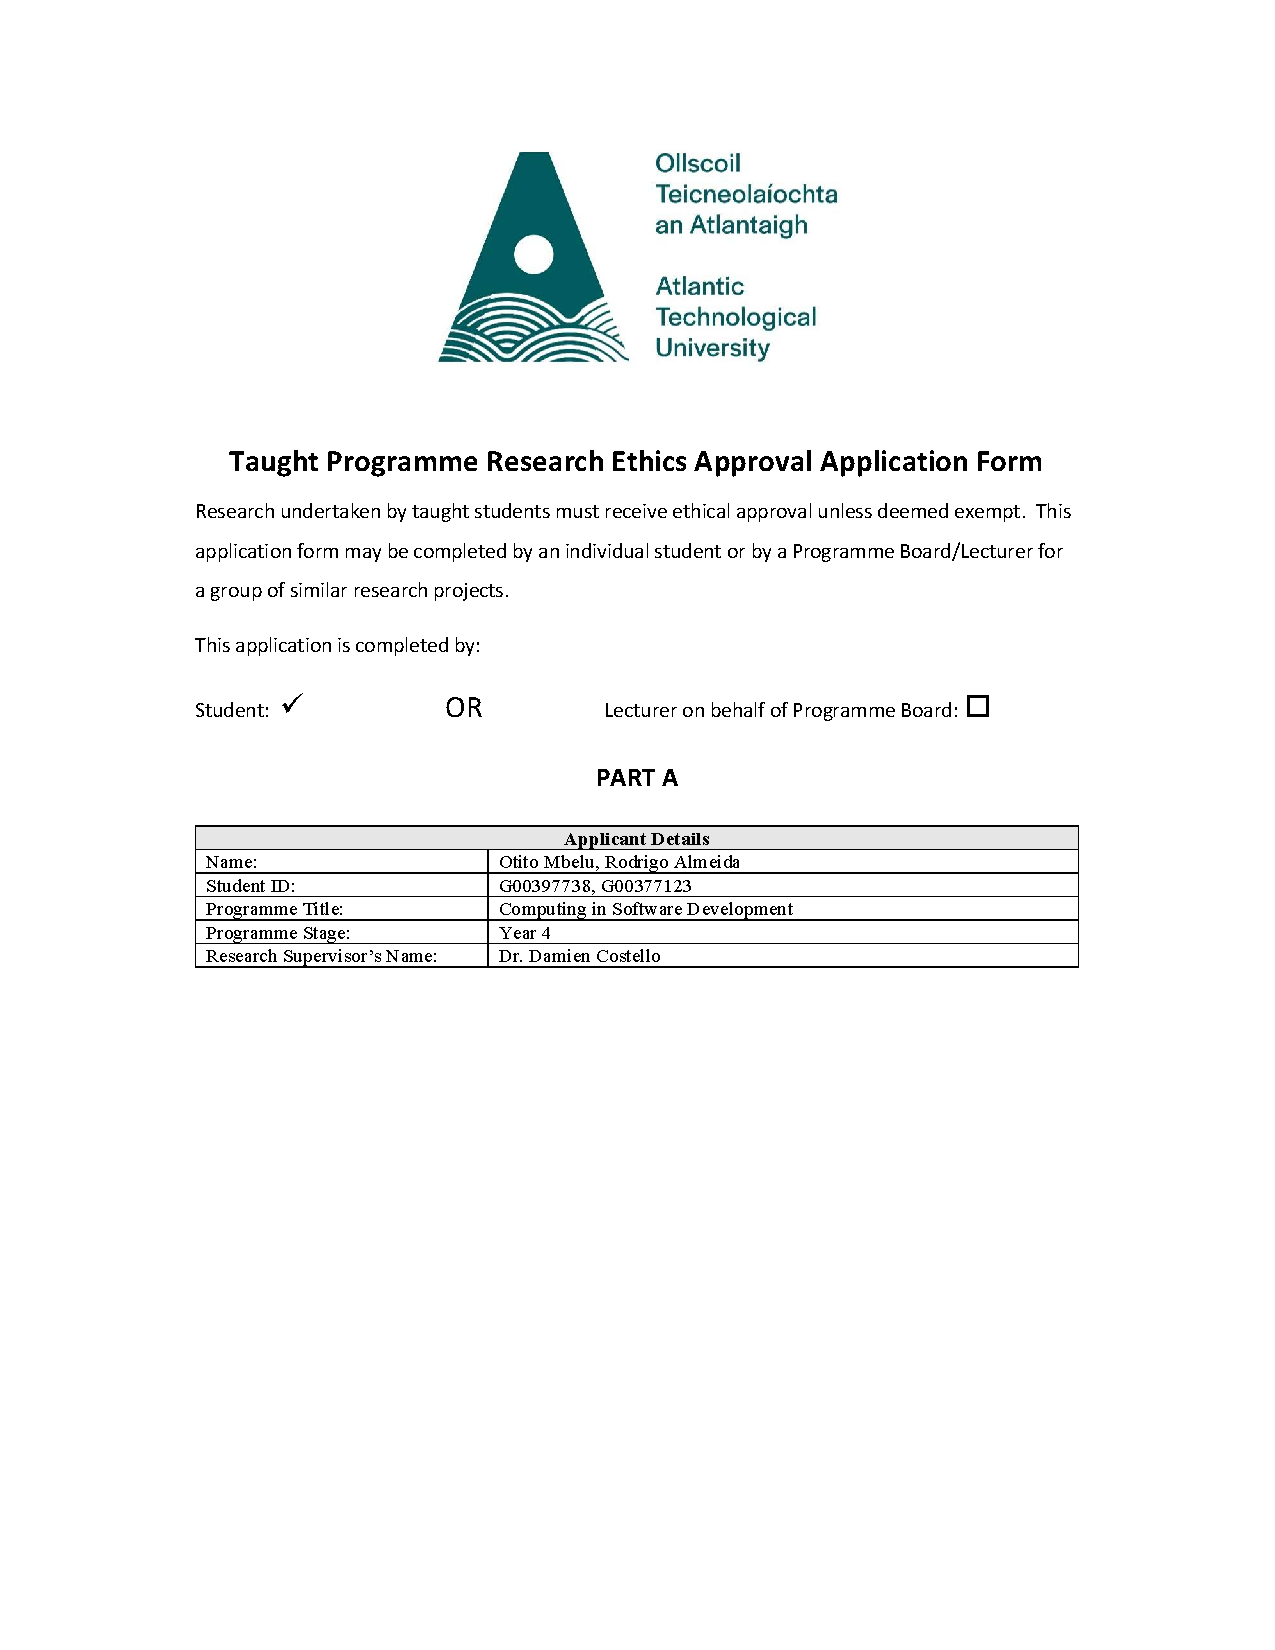
\includepdf[pages=-]{ethics_application.pdf}




\label{sec:form-recruitment}
\addcontentsline{toc}{section}{Appendix C: Microsoft Form for Volunteer Recruitment}
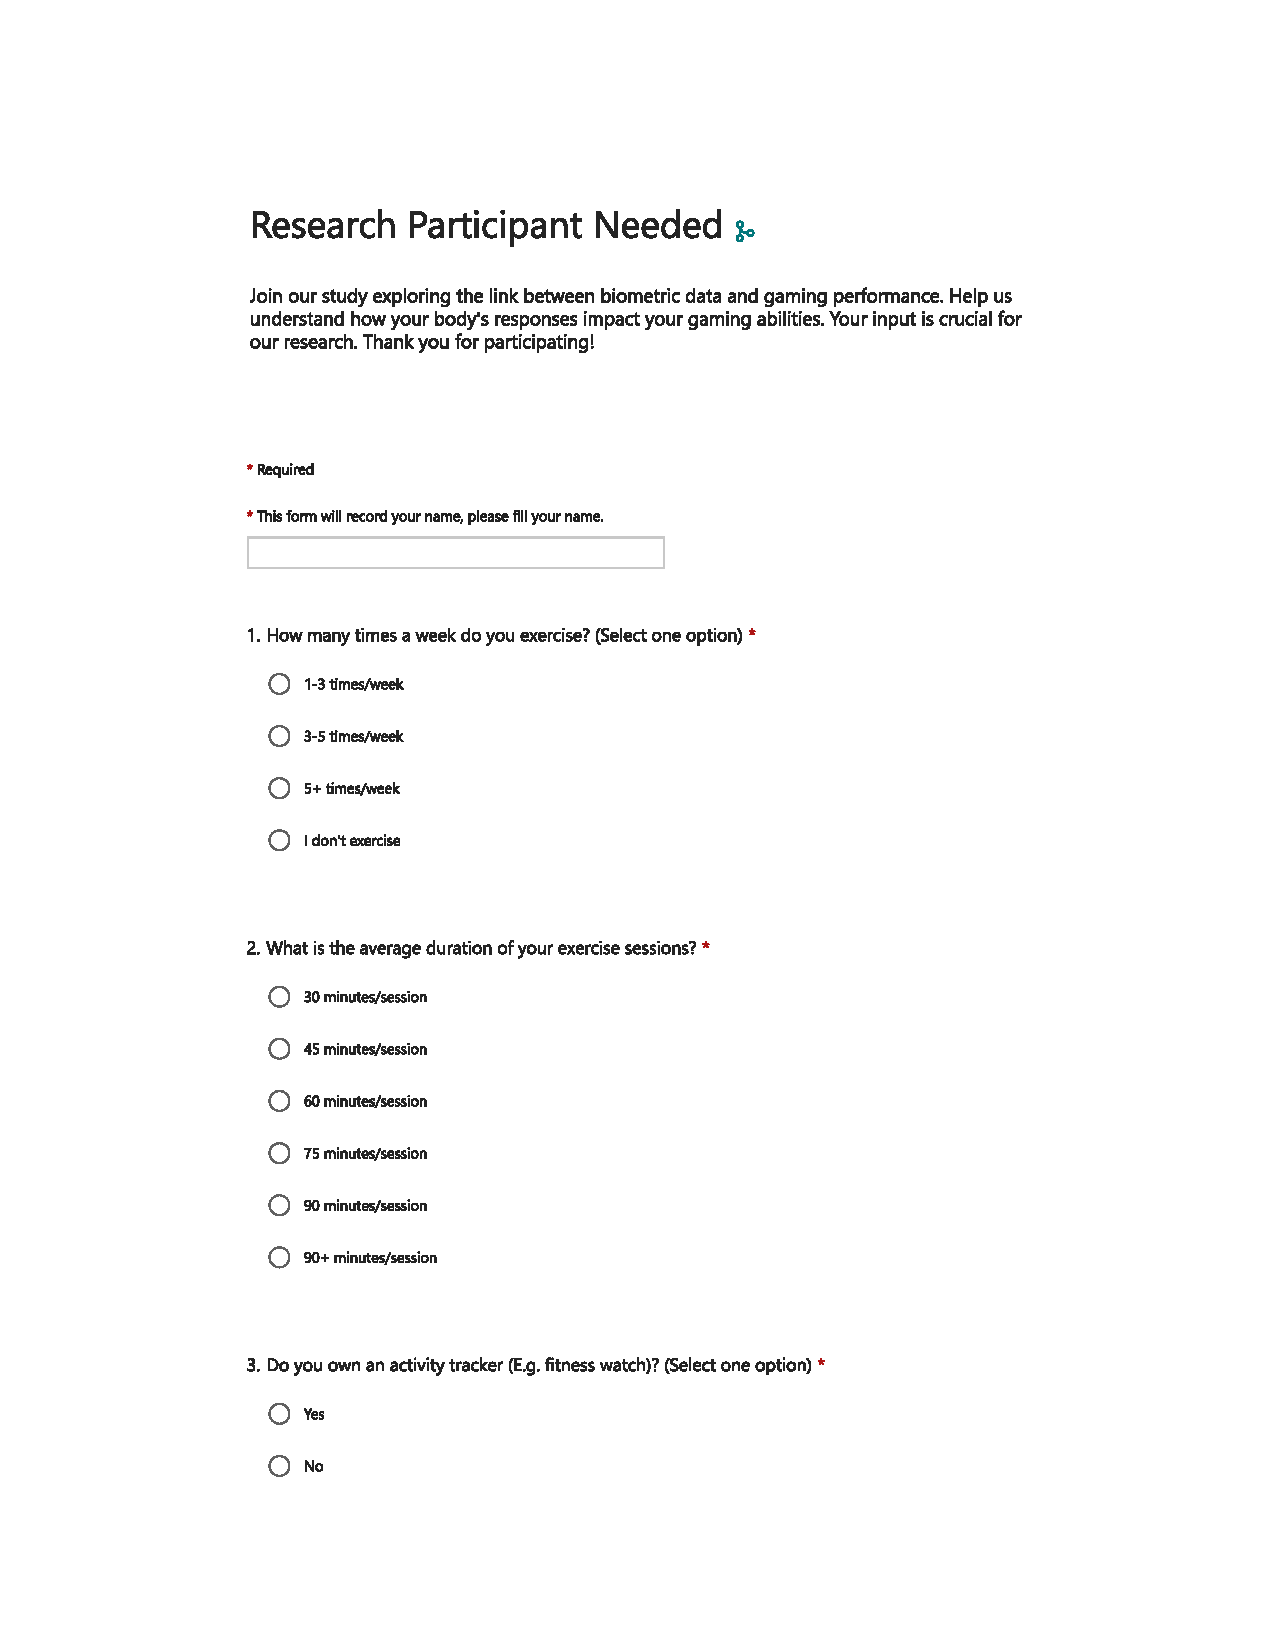
\includepdf[pages=-]{volunteer_recruitment.pdf}





%------------------------------------------------------------------------------------------------------	
% Generate the bibliography. You may have to build the document more than once before all of the
% references and processed and cited correctly.
% WARNING: Don't mess with any of the following unless you know what you are doing.
%------------------------------------------------------------------------------------------------------	
\bibliographystyle{unsrt}
\bibliography{references.bib}
\end{document}